Neste capítulo apresentará-se um resumo da teoria de superfícies mínimas em $\R^3$ e em $S^3$. 
Principalmente tomou-se como referencia as notas de aula do curso de Superfícies Mínimas ditado pelo professor Fernando Manfio no primeiro semestre do ano 2019 no Instituto de Ciências Matemáticas e de Computação da Universidade de São Paulo.
Adicionalmente, na primeira seção, tomou-se como referencia o livro de Manfredo do Carmo \cite{Carmo2010}.
As seções seguintes apresentam-se como resultados derivados da teoria de variedades riemannianas do capítulo 2 e vários artigos entre os quais o principal foi \cite{Brendle2013}.

\section{Superfícies mínimas em $\realnumbers^3$}
Nesta seção exporá-se uma introdução a teoria de superfícies mínimas em $\R^3$.
O estudo de superfícies minímas em $\R^3$ está representado pela procura de novas superfícies mínimas adicionais as já conhecidas: o catenoide e o helicoide.
O catenoide e o helicoide tem a particularidade que são as únicas superfícies mínimas rotacionais e regradas respectivamente.
O problema da procura de novas superfícies mínimas foi resolvido pelo desenvolvimento da formula de representação de Weierstrass que será mostrada na seguinte seção.
%\begin{definicao}
%	Uma superfície regular $M$ em $\realnumbers^3$ é chamada \emph{superfície mínimas} se $H(p)=0$ para qualquer $p \in M$.
%\end{definicao}
%\begin{observacao}
%	Se $H \equiv 0$, então $K_1 + K_2 \equiv 0$. Logo $K_1 = -K_2$
%\end{observacao}
%\begin{exemplo}
%	Um plano em $\realnumbers^3$ é trivialmente mínima, pois $K_1=K_2=0$.
%\end{exemplo}
%A motivação histórica do estudo das superfícies mínimas foi dada por Lagrange o ano 1760 como seguinte problema:
%Dado uma curva fechada $\gamma$ em $\realnumbers^3$, sem autointerseções, determinar a superfície de área mínima, e que tem $\gamma$ como fronteira.
%Seja $M$ uma superfície regular orientada em $\realnumbers^3$, e considere uma função $f \in \smoothfunctionsspace{M}$.
%\begin{definicao}
%	Uma \emph{variação normal} de $M$, relativa à função $f$, é uma família de superfícies $M_t$, com $t \in (-\epsilon,\epsilon)$, dadas por:
%	\begin{equation*}
%	p_t = p + t f(p) N(p),
%	\end{equation*}
%	onde $N$ é o campo unitário normal a $M$, na orientação de $M$.
%\end{definicao}
%Para $\epsilon > 0$ suficientemente pequeno, cada conjunto $M_t$ também e uma superfície regular chamada uma \emph{superfície de variação}.
%Note que para $t=0$, $M_0=M$. Se $f \equiv 1$, $M_t$ é uma superfície \emph{paralela} a $M$ a uma distancia $t$.
%**gráfico**
%Dados uma variação normal $M_t$ de $M$ relativa a uma função suave $f: M \rightarrow \realnumbers$, com $t \in (-\epsilon,\epsilon)$, e $D \subset M$ um domínio limitado, considere
%\begin{equation*}
%D_t = \{ p_t \in M_t: p \in D \}
%\end{equation*}
%para cada $t \in (-\epsilon,\epsilon)$, $D_t$ é um domínio correspondente em $M_t$. Definimos em cada $t$
%\begin{equation*}
%A(t) = \text{Area}(D_t)
%\end{equation*}
%\begin{teorema}
%	\begin{equation*}
%	A'(0) = -2 \int_D Hf dA
%	\end{equation*}
%\end{teorema}
%A expressão acima chama-se a \emph{formula da primeira variação da área}.
%\begin{demonstracao}
%	contenidos...
%\end{demonstracao}

\begin{definicao}
	Uma superfície parametrizada regular é chamada de \emph{mínima} se a sua curvatura média é identicamente nula.
\end{definicao}

\begin{definicao}
	Seja
	$x: U \subset \R^2 \rightarrow \R^3$ uma superfície parametrizada regular,
	$D \subset U$ um domínio aberto simplesmente conexo,
	$\overline{D}$ o fecho de $D$,
	$h: \overline{D} \rightarrow \R$ uma função diferenciável,
	$(u,v) \in \overline{D}$,
	$t \in (-\epsilon,\epsilon)$ e
	$N$ um campo de vetores normais unitário de $M$.
	A \emph{variação normal} de $x(\overline{D})$, determinada por $h$, é a aplicação $\varphi: \overline{D} \times (-\epsilon, \epsilon) \rightarrow \R^3$ dada por
	\begin{equation*}
		 \varphi(u,v,t) = x(u,v) + t h(u,v) N(u,v).
	\end{equation*}
\end{definicao}
Para $t \in (-\epsilon,\epsilon)$ fixado, a aplicação $x^t: \overline{D} \rightarrow \R^3$ dada por
\begin{equation}
	x^t(u,v) = \varphi(u,v,t)
\end{equation}
é uma superfície parametrizada.

Sejam $E^t, F^t, G^t$ os coeficientes da primeira forma fundamental de $x^t$.
Então, a área de $x^t(\overline{D})$ está dada por
\begin{equation*}\label{eq:3.1b}
	A(t) = \int_{\overline{D}} \sqrt{E^t G^t - (F^t)^2} du dv.
\end{equation*}
Sabe-se que
\begin{align*}
	E^t &= \innerproduct{x_u^t}{x_u^t},\\
	F^t &= \innerproduct{x_u^t}{x_v^t},\\
	G^t &= \innerproduct{x_v^t}{x_v^t}.
\end{align*}
Como $x^t(u,v) = \varphi(u,v,t)$, então
\begin{equation*}\label{eq:3.1a}
	E^t G^t - (F^t)^2 = E G - F^2 - 2 t h (Eg - 2Ff + Ge) + R,
\end{equation*}
onde $R$ é un resto tal que $\lim_{t \rightarrow 0} R/t = 0$.
Dado que
\begin{equation*}
	H = \frac{1}{2} \left(\frac{Eg - 2Ff + Ge}{E G - F^2}\right)
\end{equation*}
então, \eqref{eq:3.1a} pode-se escrever
\begin{equation*}
	E^t G^t - (F^t)^2 = (EG - F^2)(1 - 4thH) + R
\end{equation*}
Finalmente a equação \eqref{eq:3.1b} escreve-se
\begin{equation*}
	A(t) = \int_{\overline{D}} \sqrt{1 - 4thH + \overline{R}} \sqrt{EG - F^2} du dv
\end{equation*}
onde $\overline{R} = R/\sqrt{EG - F^2}$.
Derivando $A(t)$ em $t=0$ tem-se
\begin{equation*}\label{eq:3.1c}
	A'(0) = -\int_{\overline{D}} 2hH \sqrt{EG - F^2} du dv
\end{equation*}

\begin{proposicao}\label{caracteristica_das_superficies_minimas}
	Uma superfície $M$ em $\realnumbers^3$ é mínima se e somente se $A'(0) = 0$.
\end{proposicao}

\begin{demonstracao}
	Supondo que a superfície é mínima então, pela equação \eqref{eq:3.1c}, tem-se que $A'(0) = 0$.
	Agora supor que existe $p \in \overline{D}$ tal que $H(p) \neq 0$. 
	Seja $U \subset \overline{D}$ aberto tal que $p \in U$. 
	Pelo fato que a função $h$ é arbitraria, pudemos escolher $h: \overline{D} \rightarrow \R$ tal que $h(p) = H(p)$, $hH > 0$ em  $U$, e $h$ seja identicamente nula fora $U$. 
	Com as condições anteriores, tem-se que $A'(0) < 0$.
\end{demonstracao}
%\begin{observacao}
	Suponha que exista uma solução $M$ para o problema de Lagrange, e considere uma variação normal $M_t$ de $M$, com $t \in (-\epsilon,\epsilon)$, dada por uma função suave $f: M \rightarrow \realnumbers$ tal que $f_{|\partial M} = 0$. Como a área de $M$ é mínima temos, em particular, que
	\begin{equation*}
	A(t) \geq A(0)
	\end{equation*}
	para qualquer $t \in (-\epsilon,\epsilon)$. Portanto, $A'(0)=0$, para toda variação normal $M_t$ de $M$ com $f_{|\partial M}=0$.
	Isso mostra, em virtude da proposição \ref{caracteristica_das_superficies_minimas}, que as superfícies de área mínima são superfícies mínimas no sentido da nossa definição. A reciproca é falsa!
%\end{observacao}

\begin{proposicao}
	Não existe superfície minima compacta em $\realnumbers^3$.
\end{proposicao}

\begin{demonstracao}
	Se $M$ é minima, então
	\begin{equation*}
	H = \frac{1}{2} (k_1 + k_2) = 0.
	\end{equation*}
	Logo $k_1 = -k_2$ e se tem que $K = k_1 k_2 \leq 0$.
	Se $M$ for compacta, existe $p \in M$ tal que $K(p) > 0$.
\end{demonstracao}
Dada suma superfície regular $M$ em $\realnumbers^3$, considere uma carta local isoterma $(U,\varphi)$ para $M$, i.e., 
\begin{equation*}
E = G = \lambda^2 \text{ e } F=0,
\end{equation*}
onde $\lambda: U \rightarrow \realnumbers$ é uma função diferenciável com $\lambda > 0$. Note que, nas coordenadas isotermas $\varphi \sim (x,y)$, a curvatura media se expressa como
\begin{align*}
H &= \frac{eG - 2fF + gE}{2(EG - F^2)}\\
&= \frac{e + g}{2 \lambda^2}
\end{align*}

\begin{definicao}
	Dado uma função diferenciável $f: U \subset \realnumbers^2 \rightarrow \realnumbers$, o \emph{Laplaciano} de $f$, denotado por $\Delta f$, é definido por
	\begin{equation*}
	\Delta f = \frac{\partial^2 f}{\partial x^2} + \frac{\partial^2 f}{\partial y^2}.
	\end{equation*}
	Dizemos que $f$ é \emph{harmônica} se $\Delta f = 0$.
	Se $(U, \varphi)$ é uma carta local para $M$ como $\varphi = (\varphi_1, \varphi_2, \varphi_3)$, definimos
	\begin{equation*}
	\Delta \varphi = (\Delta \varphi_1, \Delta \varphi_2, \Delta \varphi_3).
	\end{equation*}
\end{definicao}

\begin{proposicao}
	Se $(U, \varphi)$ é uma carta local isoterma em $M$, então 
	\begin{equation*}
	\Delta \varphi = 2 \lambda^2 H N
	\end{equation*}
\end{proposicao}

\begin{demonstracao}
	Como $\varphi$ é isoterma, com $\varphi \sim (u, v)$, temos
	\begin{gather*}
	\innerproduct{\varphi_u}{\varphi_v} = \lambda^2 = \innerproduct{\varphi_v}{\varphi_u} \\
	\text{ e } \innerproduct{\varphi_u}{\varphi_v} = 0
	\end{gather*}
	Derivando, obtemos:
	\begin{align*}
	\innerproduct{\varphi_{uu}}{\varphi_u} &= \innerproduct{\varphi_{vu}}{\varphi_v}\\
	&= - \innerproduct{\varphi_u}{\varphi_{vv}}
	\end{align*}
	Disso decorre que
	\begin{equation}\label{eq1}
	\innerproduct{\varphi_{uu} + \varphi_{vv}}{\varphi_u} = 0
	\end{equation}
	Analogamente, obtemos:
	\begin{equation}\label{eq2}
	\innerproduct{\varphi_{uu} + \varphi_{vv}}{\varphi_v} = 0
	\end{equation}
	De \eqref{eq1} e \eqref{eq2} concluímos que $\varphi_{uu} + \varphi_{vv}$ é paralela a $N$. Alem disso, como
	\begin{equation}
	H = \frac{e+g}{2 \lambda^2}
	\end{equation}
	obtemos:
	\begin{align*}
	2 \lambda^2 H &= e + g = \innerproduct{\varphi_{uu}}{N} + \innerproduct{\varphi_{vv}}{N}\\
	&= \innerproduct{\varphi_{uu} + \varphi_{vv}}{N}.
	\end{align*}
	Isso mostra que
	\begin{equation}
	\Delta \varphi = 2 \lambda^2 H N
	\end{equation}
\end{demonstracao}

\begin{corolario}\label{equiv_isoterma_harmonica}
	Uma superfície $M$ em $\realnumbers^3$ é mínima se e somente se toda carta local isoterma é harmônica.
\end{corolario}

\begin{exemplo}
	O \emph{catenoide} é a superfície em $\realnumbers^3$ gerada pela rotação da catenária 
	\begin{equation*}
	y = a \cosh \left( \frac{z}{a} \right)
	\end{equation*}
	em torno ao eixo $z$.
	Assim, o catenoide pode ser parametrizado por
	\begin{equation*}
	\varphi(u,v) = \left( a \cosh v \cos u, a \cosh v \sin u, av \right)
	\end{equation*}
	onde $u \in (0, 2 \pi)$ e $v \in \realnumbers$. Para tal $\varphi$, obtemos
	\begin{gather*}
	E = G = a^2 \cosh^2 v,\\
	F = 0,\\
	\varphi_{uu} + \varphi_{vv} = 0.
	\end{gather*}
	Portanto o catenoide e uma superfície minima.
\end{exemplo}

\begin{figure}
	\centering
	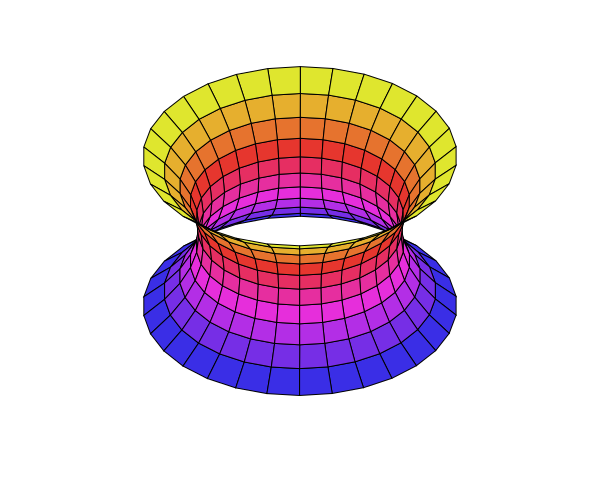
\includegraphics[width=0.5\textwidth]{images/catenoid}
	\caption{Catenoide. Imagem obtida de \url{https://upload.wikimedia.org/wikipedia/commons/5/5d/Catenoid.svg} baixo licença Creative Commons.}
\end{figure}

\begin{exemplo}
	Considere uma hélice dada por
	\begin{equation*}
	\alpha(u) = \left( \cos u, \sin u, au \right).
	\end{equation*}
	Por cada ponto da hélice, trace uma reta paralela ao plano $XY$ que intercepta o eixo $Z$.
	(Gráfico)
	A superfície gerada por tais retas é o \emph{helicoide} e pode ser parametrizada por
	\begin{equation*}
	\varphi(u,v) = \left( v \cos u, v \sin u, au \right)
	\end{equation*}
	com $u \in (0, 2 \pi)$ e $v \in \realnumbers$. Temos
	\begin{gather*}
	E = G = a^2 \cosh^2 v\\
	F = 0\\
	\varphi_{uu} + \varphi_{vv} = 0.
	\end{gather*}
	Portanto o helicoide é superfície minima.
\end{exemplo}

\begin{figure}
	\centering
	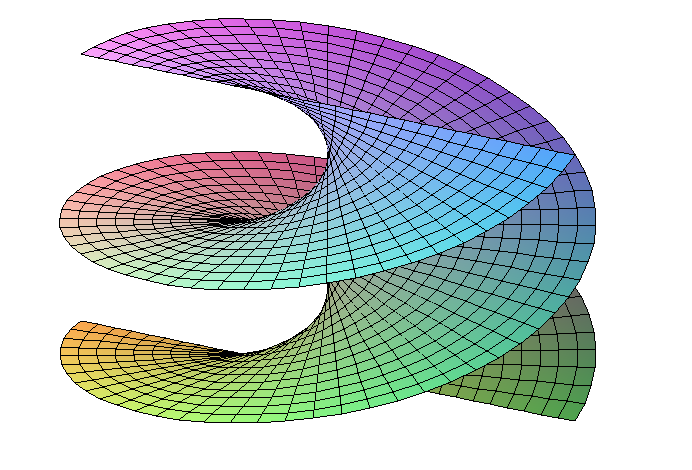
\includegraphics[width=0.5\textwidth]{images/helicoid}
	\caption{Helicoide. Imagem obtida de \url{https://upload.wikimedia.org/wikipedia/commons/d/d2/Helicoid_JD.png} baixo licença Creative Commons.}
\end{figure}

\begin{teorema}
	Alem do plano,
	\begin{enumerate}
		\item[a)] O catenoide é a única superfície rotacional minima.
		\item[b)] O helicoide é a única superfície regrada minima.
	\end{enumerate}
\end{teorema}

\begin{demonstracao}
	Para a demonstração de $a)$, ver \cite[§3.5, Exemplo 5]{Carmo2010}. 
	Para a demonstração de $b)$, ver \cite[§3.5, Exemplo 6]{Carmo2010}.
\end{demonstracao}

\begin{exemplo}
	Dado uma função diferenciável $f: U \rightarrow \realnumbers$, definida num aberto $U \subset \realnumbers^2$, considere o gráfico $\text{Gr}(f)$ de $f$, parametrizado por
	\begin{equation*}
	\varphi(x,y) = (x,y,f(x,y)), (x,y) \in U.
	\end{equation*}
	Temos
	\begin{align*}
	\varphi_x &= (1,0,f_x)\\
	\varphi_y &= (0,1,f_y).
	\end{align*}
	Assim
	\begin{align*}
	E &= \innerproduct{\varphi_x}{\varphi_x} = 1 + f_x^2\\
	F &= \innerproduct{\varphi_x}{\varphi_y} = f_x f_y\\
	G &= \innerproduct{\varphi_y}{\varphi_y} = 1 + f_y^2.
	\end{align*}
	Un campo $n$, normal a $\text{Gr}(f)$, é dado por
	\begin{align*}
	n = \varphi_x \times \varphi_y &= \det \left[ \begin{matrix}
	i & j & k\\
	1 & 0 & f_x\\
	0 & 1 & f_y
	\end{matrix} \right]\\
	&= (-f_x, -f_y, 1).
	\end{align*}
	Normalizando, temos
	\begin{equation*}
	N = \frac{n}{\norm{n}} = \frac{1}{\sqrt{1 + f_x^2 + f_y^2}}(-f_x, -f_y, 1).
	\end{equation*}
	Como
	\begin{align*}
	\varphi_{xx} &= (0, 0, f_{xx})\\
	\varphi_{xy} &= (0, 0, f_{xy})\\
	\varphi_{yy} &= (0, 0, f_{yy})
	\end{align*}
	obtemos
	\begin{align*}
	e &= \innerproduct{\varphi_{xx}}{N} = \frac{f_{xx}}{\sqrt{1 + f_x^2 + f_y^2}}\\
	f &= \innerproduct{\varphi_{xy}}{N} = \frac{f_{xy}}{\sqrt{1 + f_x^2 + f_y^2}}\\
	g &= \innerproduct{\varphi_{yy}}{N} = \frac{f_{yy}}{\sqrt{1 + f_x^2 + f_y^2}}.
	\end{align*}
	Assim, como
	\begin{equation*}
	H = \frac{eG - 2fF + gE}{2(EG - F^2)}
	\end{equation*}
	segue que se $H \equiv 0$, temos
	\begin{equation}\label{edp_superficies_minimas}
	(1 + f_y^2) f_{xx}  - 2 f_x f_y f_{xy} + (1+f_x^2) f_{yy} = 0
	\end{equation}
	que é uma EDP de 2da ordem.
	Um exemplo trivial da equação \ref{edp_superficies_minimas} é a função linear
	\begin{equation*}
	f(x,y) = ax + by + c,
	\end{equation*}
	como $a, b, c \in \realnumbers$.
\end{exemplo}

\begin{exemplo}[Superfície de Scherk]
	Suponha que
	\begin{equation*}
	f(x,y) = g(x) + h(y).
	\end{equation*}
	Neste caso, a equação \ref{edp_superficies_minimas} pode ser escrita como
	\begin{equation*}
	(1 + (h')^2(y)) g''(x) + (1 + (g')^2(x)) h''(y) = 0,
	\end{equation*}
	ou seja
	\begin{equation*}
	\frac{g''(x)}{1 + (g')^2(x)} + \frac{h''(y)}{1 + (h')^2(y)} = 0.
	\end{equation*}
	Isso implica
	\begin{equation*}
	\frac{g''(x)}{1 + (g')^2(x)} = - \frac{h''(y)}{1 + (h')^2(y)} = \text{constante}.
	\end{equation*}
	Integrando, obtemos (a menos de constantes) que
	\begin{align*}
	g(x) &= \ln (\cos x)\\
	h(y) &= -\ln (\cos y).
	\end{align*}
	A menos de dilatações e translações uma parte da superfície pode ser representada pelo gráfico da função
	\begin{equation*}
	\ln \left( \frac{\cos x}{\cos y} \right), 0 < x,y < \frac{\pi}{2}
	\end{equation*}
\end{exemplo}

\begin{figure}
	\centering
	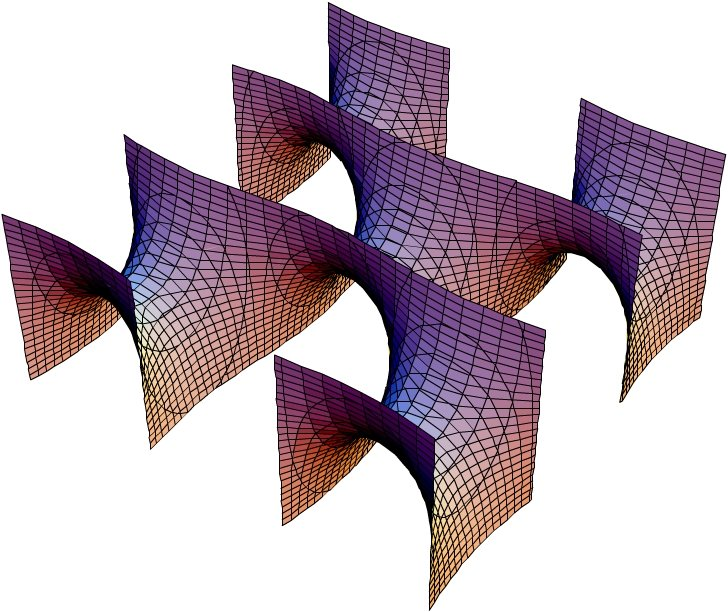
\includegraphics[width=0.5\textwidth]{images/scherk}
	\caption{Superfície de Scherk. Imagem obtida de \url{https://upload.wikimedia.org/wikipedia/commons/8/83/Superficie_di_scherk.jpg} baixo licença Creative Commons.}
\end{figure}

\section{A formula de representação de Weierstrass}
Nesta seção apresentará-se a formula de representação de Weierstrass que serve para gerar superfícies mínimas em $\R^3$. Este foi um problema importante ao inicio do estúdio das superfícies mínimas.
Esta formula faz uso da teoria de superfícies de Riemann e Analise Complexa.

Considere o plano complexo $\complexnumbers$ identificado com $\realnumbers^2$
\begin{equation*}
(x,y) \in \realnumbers^2 \mapsto x + iy \in \complexnumbers.
\end{equation*}
Uma função complexa $f: U \subset \complexnumbers \rightarrow \complexnumbers$ pode ser escrita na forma
\begin{equation*}
f(u,v) = f_1(u,v) + i f_2(u,v)
\end{equation*}
onde $f_1, f_2: U \rightarrow \realnumbers$ são funções reais, denotadas por
\begin{align*}
f_1 &= \Re(f)\\
f_2 &= \Im(f)
\end{align*}
tal que $\Re(f)$ é parte real da função $f$ e $\Im(f)$ é a parte imaginaria da função $f$.
\begin{definicao}
	Uma função $f: U \subset \complexnumbers \rightarrow \complexnumbers$, definida no aberto $U$, é dita \emph{holomorfa} se $f_1, f_2$ possuem derivadas parciais continuas e satisfazem as equações de Cauchy-Riemann
	\begin{align*}
	\partialdifffrac{f_1}{u} &= \partialdifffrac{f_2}{v}\\
	\partialdifffrac{f_1}{v} &= - \partialdifffrac{f_2}{u}
	\end{align*}
\end{definicao}

%\begin{definicao}
%	Uma carta local $(U, \varphi)$ em $M$ é dita \emph{mínima} se $H(p) = 0, \forall p \in \varphi(U)$.
%\end{definicao}

%\begin{corolario}
%	Seja $(U, \varphi)$ uma carta local isoterma de uma superfície $M \subset \realnumbers^3$. Então $(U, \varphi)$ é mínima se e somente se $\varphi$ é harmônica, i.e., $\varphi_{uu} + \varphi_{vv} = 0$.
%\end{corolario}

Dadas uma superfície $M \subset \realnumbers^3$ e uma carta local $(U, \varphi)$ em $M$, com
\begin{equation*}
\varphi(u,v) = (x_1(u,v), x_2(u,v), x_3(u,v)),
\end{equation*}
considere as funções complexas $f_j: U \subset \complexnumbers \rightarrow \complexnumbers, 1 \leq j \leq 3,$ dadas por
\begin{equation}\label{carta_isoterma_cauchy-riemann}
f_j = \partialdifffrac{x_j}{u} - i \partialdifffrac{x_j}{v}, 1 \leq j \leq 3
\end{equation}

\begin{lema}
	Seja $(U, \varphi)$ uma carta local isoterma em $M$. Então, $\varphi$ é mínima se e somente se cada $f_j$, definida em \eqref{carta_isoterma_cauchy-riemann}, é holomorfa.
\end{lema}

\begin{demonstracao}
	Pelo corolário \ref{equiv_isoterma_harmonica}, temos que $\varphi$ é mínima se e somente se $\varphi$ é harmônica, i.e., $\varphi_{uu} + \varphi_{vv} = 0$. Isso significa que
	\begin{equation*}
	\npartialdifffrac{x_j}{u}{2} + \npartialdifffrac{x_j}{v}{2} = 0, 1 \leq j \leq 3.
	\end{equation*}
	Queremos provar que
	\begin{align*}
	\pdiff{u} \Re(f_j) &= \pdiff{v} \Im(f_j),\\
	\pdiff{v} \Re(f_J) &= - \pdiff{u} \Im(f_j)
	\end{align*}
	Assim
	\begin{equation*}
	\pdiff{u} \Re(f_J) = \pdiff{u} \partialdifffrac{x_j}{u} = \npartialdifffrac{x_j}{u}{2} = - \npartialdifffrac{x_j}{v}{2} = \pdiff{v} \left( - \partialdifffrac{x_j}{v} \right) = \pdiff{v} \Im(f_j)
	\end{equation*}
	Isso prova a primeira equação de Cauchy-Riemann. Por outro lado, como a superfície é regular, vale
	\begin{equation*}
	\varphi_{uv} = \varphi_{vu},
	\end{equation*}
	ou seja
	\begin{equation*}
	\frac{\partial^2 x_j}{\partial u \partial v} = \frac{\partial^2 x_j}{\partial v \partial u}.
	\end{equation*}
	Assim
	\begin{align*}
	\pdiff{v} \Re(f_j) &= \pdiff{v} \partialdifffrac{x_j}{u} = \pdiff{u} \partialdifffrac{x_j}{v}\\
	&= \pdiff{u} \left( - \Im(f_j) \right)\\
	&= - \pdiff{u} \Im(f_j),
	\end{align*}
	que é a segunda equação de Cauchy-Riemann.
\end{demonstracao}

\begin{lema}\label{lema_fj_2}
	Sejam $M \subset \realnumbers^3$ uma superfície mínima e $(U, \varphi)$ uma carta local isoterma. Então, as funções holomorfas $f_j$, definidas em \eqref{carta_isoterma_cauchy-riemann}, satisfazem
	\begin{gather}\label{sum_fj_2}
	f_1^2 + f_2^2 + f_3^2 = 0\\ \label{sum_norm_fj_2}
	|f_1|^2 + |f_2|^2 + |f_3|^2 \neq 0
	\end{gather}
	Reciprocamente, sejam $f_1, f_2, f_3$ funções holomorfas, definidas num aberto simplesmente conexo $U \subset \complexnumbers$, satisfazendo \eqref{sum_fj_2} e \eqref{sum_norm_fj_2}. Então, tais funções dão origem a uma carta local isoterma mínima $(U, \varphi)$.
\end{lema}

\begin{demonstracao}
	Seja $(U, \varphi)$ a carta local isoterma em $M$. Então,
	\begin{align*}
	f_1^2 + f_2^2 + f_3^2 &= \sum_{j=1}^{3} \left[ \left( \partialdifffrac{x_j}{u} \right)^2 - \left( \partialdifffrac{x_j}{v} \right)^2 - 2i \partialdifffrac{x_j}{u} \partialdifffrac{x_j}{v} \right]\\
	&= E - G - 2iF = 0,
	\end{align*}
	pois $E=G$ e $F=0$. A equação \eqref{sum_norm_fj_2} segue da regularidade de $\varphi$, pois $\varphi_u \neq 0$ e $\varphi_v \neq 0$.
	Reciprocamente, defina
	\begin{equation}\label{carta_isoterma_eq_integral}
	x_j(u,v) = \int_{\xi_0}^{\xi} f_j(z) dz, 1 \leq j \leq 3
	\end{equation}
	com $\xi = (u,v) \in U$, para algum $\xi_0 \in U$ fixado. Note que cada $x_j$ está bem definida pois $U$ é simplesmente conexo e $f_j$ é holomorfa, o que nos dá uma função holomorfa definida em $U$, para o qual podemos aplicar as equações de Cauchy-Riemann, obtendo:
	\begin{align*}
	\frac{d}{d \xi} \int_{\xi_0}^{\xi} f_j &= \frac{d}{d \xi} \left[ \Re \int_{\xi_0}^{\xi} f_j + i \Im \int_{\xi_0}^{\xi} f_j \right]\\
	&= \pdiff{u} \Re \int_{\xi_0}^{\xi} f_j + i \pdiff{u} \Im \int_{\xi_0}^{\xi} f_j\\
	&= \pdiff{u} \Re \int_{\xi_0}^{\xi} f_j - i \pdiff{v} \Re \int_{\xi_0}^{\xi} f_j
	\end{align*}
	de modo que a equação \eqref{carta_isoterma_cauchy-riemann} é válida. Considere a aplicação $\varphi: U \rightarrow \realnumbers^3$, cujas funções coordenadas
	\begin{equation*}
	\varphi = (x_1,x_2,x_3)
	\end{equation*}
	são dadas como em \eqref{carta_isoterma_eq_integral}. De \eqref{sum_fj_2} e \eqref{sum_norm_fj_2} segue que $(U,\varphi)$ é uma carta local isoterma. Além disso, as funções $f_j$ serem holomorfas implicam que as funções coordenadas $x_j$ são harmônicas, logo, pelo corolário, $\varphi$ é mínima.
\end{demonstracao}

\begin{observacao}
	As funções $x_j$ definidas em \eqref{carta_isoterma_eq_integral} estão definidas a menos de uma constante aditiva, de modo que a superfície está definida a menos de uma translação. Assim, o estudo local de superfícies mínimas em $\realnumbers^3$ reduz-se a resolver as equações \eqref{sum_fj_2} e \ref*{sum_norm_fj_2} para uma terna de funções holomorfas.
\end{observacao}

\begin{teorema}
	Sejam $f: U \subset \complexnumbers \rightarrow \complexnumbers$ uma função holomorfa e $g: U \rightarrow \complexnumbers$ uma função meromorfa tais que $fg^2$ seja holomorfa. Assuma que se $\xi \in U$ é um polo de ordem $n$ para $g$ então $\xi$ é um zero para $f$ de ordem $2n$, e que estes sejam os únicos zeros de $f$.
	Então, a aplicação
	\begin{equation}\label{carta_minima_duas_funcoes}
	\varphi(z) = \frac{1}{2} f(z) \left( (1-g(z)^2), i (1+g(z)^2), 2g(z) \right)
	\end{equation}
	satisfaz as condições do Lema \ref{lema_fj_2}. Além disso, para toda tal $\varphi$, existem funções holomorfa $f$ e meromorfa $g$ tais que vale \eqref{carta_minima_duas_funcoes}.
\end{teorema}

\begin{demonstracao}
	Se $\varphi$ satisfaz \eqref{carta_minima_duas_funcoes}, temos
	\begin{align*}
	f_1^2 + f_2^2 + f_3^2 &= \frac{1}{4} f(z)^2 (1 - g(z)^2)^2 - \frac{1}{4} f(z)^2 (1 + g(z)^2)^2 + f(z)^2 g(z)^2\\
	&= 0
	\end{align*}
	Afirmamos que $\varphi(z) \neq 0, \forall z \in U$. De fato, a hipótese sobre os zeros de $f$ e os polos de $g$ implicam que $f(z) g(z)^2 \neq 0$. Assim, para qualquer $z$ fixado, a primeira e a segunda coordenada de $\varphi$ não podem ser ambas nulas.
	Assim, podemos assumir que $\varphi$ é holomorfa satisfazendo
	\begin{equation*}
	\varphi_1^2 + \varphi_2^2 + \varphi_3^2 \not\equiv 0,
	\end{equation*}
	$\varphi$ nunca é zero, e considere
	\begin{align*}
	f(z) &= \varphi_1(z) - i \varphi_2(z)\\
	g(z) &= \frac{\varphi_3(z)}{\varphi_1(z) - i \varphi_2(z)}
	\end{align*}
	$f$ é uma função holomorfa e $g$ é o quociente de funções holomorfas. Se o denominador de $g$ é identicamente nulo, façamos
	\begin{equation*}
	g(z) = \frac{\varphi_3(z)}{\varphi_1(z) + i \varphi_2(z)}
	\end{equation*}
	e proceder de forma similar.
	Assim, sendo o denominador de $g$ não nulo, tem-se que $g$ é meromorfa. Assim, a relação
	\begin{equation*}
	\varphi_1^2 + \varphi_2^2 + \varphi_3^2 = 0
	\end{equation*}
	implica
	\begin{equation*}
	(\varphi_1 + i \varphi_2)(\varphi_1 - i \varphi_2) = -\varphi_3^2
	\end{equation*}
	que, em termos de $f$ e $g$ torna-se
	\begin{align*}
	\varphi_1 + i \varphi_2 &= \frac{-\varphi_3^2}{\varphi_1 - i \varphi_2}\\
	&= \frac{-\varphi_3^2}{(\varphi_1 - i \varphi_2)^2} (\varphi_1 - i \varphi_2)\\
	&= -fg^2
	\end{align*}
	Esta última equação, juntamente com as condições sobre $f$ e $g$, nos dão $\varphi$ como em \eqref{carta_minima_duas_funcoes}.
\end{demonstracao}

\begin{definicao}
	Sejam $U \subset \complexnumbers$ um aberto simplesmente conexo e $\gamma \subset U$ uma curva de um ponto fixado $z_0 \in U$ a um ponto arbitrário $z \in U$, $z = u + iv$.
	Sejam $f,g$ como no teorema anterior. Então,
	\begin{equation*}
	\varphi(u,v) = (x_1(u,v), x_2(u,v), x_3(u,v)),
	\end{equation*}
	onde
	\begin{align*}
	x_1 &= \Re \int_{\gamma} \frac{1}{2} f(z) (1 - g(z)^2) dz\\
	x_2 &= \Re \int_{\gamma} \frac{1}{2} f(z) (1 + g(z)^2) dz\\
	x_3 &= \Re \int_{\gamma} f(z) g(z) dz
	\end{align*}
	é uma carta local mínima, chamada \emph{a representação de Weierstrass} da teoria local de superfícies mínimas.
\end{definicao}

\begin{exemplo}[Catenoide]
	O catenoide pode ser representado pelas funções holomorfas $f, g: \complexnumbers \rightarrow \complexnumbers$ dadas por
	\begin{align*}
	f(z) &= e^{-z},\\
	g(z) &= e^z.
	\end{align*}
	Substituindo tais funções na formula da representação de Weierstrass e integrando de $z_0 = 0$ a um ponto arbitrário $z = u + iv$, obtemos
	\begin{align*}
	\varphi(u,v) &= x_0 + \Re \int_{z_0}^{z} \frac{f(\xi)}{2} (1 - g(\xi)^2, i (1 + g(\xi)^2), 2 g(\xi)) d\xi\\
	&= x_0 + \Re \int_{z_0}^{z} \frac{e^{-\xi}}{2} (1 - e^{2\xi}, i (1 + e^{2\xi}), 2e^{\xi}) d\xi\\
	&= \Re \int_{0}^{z} \frac{1}{2} (e^{-\xi} - e^{\xi}, i (e^{-\xi} + e^{\xi}), 1) d\xi\\
	&= \Re \left[ \frac{1}{2} \left(-e^{-z} - e^z, -\frac{1}{2i} (-e^{-z} + e^z), z \right) \right] \\
	&= \Re \left( -\cosh z, i \sinh z, z \right) \\
	&= \left( -\cosh u \cos v, -\cosh u \sin v, u \right)
	\end{align*} 
\end{exemplo}

\begin{exemplo}[Superfície de Enneper]
	A superfície de Enneper pode ser representada pelas funções holomorfas $f,g: \complexnumbers \rightarrow \complexnumbers$ dadas por
	\begin{align*}
	f(z) &= 1, \\
	g(z) &= z.
	\end{align*}
	Assim, a representação de Weierstrass torna-se
	\begin{align*}
	\varphi(u,v) &= \Re \left( \frac{1}{2} \int_{0}^{z} \left( 1 - \xi^2, i (1 + \xi^2), 2\xi \right) \right) d\xi \\
	&= \frac{1}{2} \Re \left( z - \frac{z^3}{3}, iz + \frac{iz^3}{3}, z^2 \right) \\
	&= \frac{1}{2} \left( u - \frac{u^3}{3} + uv^2, -v + \frac{v^3}{3} - u^2v, u^2 - v^2 \right)
	\end{align*}
\end{exemplo}

\begin{figure}
	\centering
	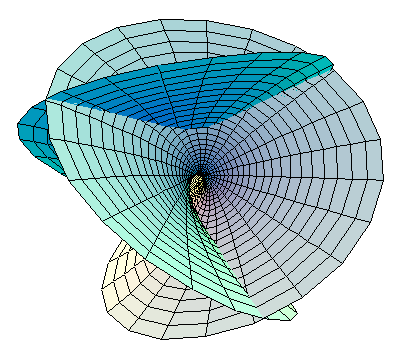
\includegraphics[width=0.5\textwidth]{images/enneper}
	\caption{Superfície de Enneper. Imagem obtida de \url{https://upload.wikimedia.org/wikipedia/commons/d/dc/EnneperSurface.PNG} baixo licença GNU Free Documentation License.}
\end{figure}

\begin{exemplo}[Superfície de Scherk]
	A superfície de Scherk, definida pela equação
	\begin{equation*}
	e^z = \frac{\cos y}{\cos x},
	\end{equation*}
	pode ser representada pelas funções holomorfas $f: \complexnumbers \setminus \{\pm 1, \pm i \} \rightarrow \complexnumbers$ e $g: \complexnumbers \rightarrow \complexnumbers$ dadas por
	\begin{align*}
	f(z) &= \frac{2}{1 - z^4}, \\
	g(z) &= z.
	\end{align*}
	Note que
	\begin{align*}
	f (1 - g^2) &= \frac{2}{1 + z^2} = \frac{i}{z + i} - \frac{i}{z - i}, \\
	i f (1 + g^2) &= \frac{2i}{1 - z^2} = \frac{i}{z + 1} - \frac{i}{z - 1}, \\
	2fg &= \frac{4z}{1 - z^4} = \frac{2z}{z^2 + 1} - \frac{2z}{z^2 - 1}.
	\end{align*}
	Assim, substituindo na representação de Weierstrass e integrando, obtemos
	\begin{equation*}
	\varphi(z) = \left( -\arg \frac{z + i}{z - i}, -\arg \frac{z + i}{z - i}, \log \left\| \frac{z^2 + 1}{z^2 - 1} \right\| \right).
	\end{equation*}
	Usando as identidades
	\begin{align*}
	\frac{z + i}{z - i} &= \frac{|z|^2 - 1}{|z^2 - i|^2} + i \frac{z + \overline{z}}{|z - i|^2}, \\
	\frac{z + 1}{z - 1} &= \frac{|z|^2 - 1}{|z - 1|^2} + i \frac{\overline{z} - z}{|z - 1|^2},
	\end{align*}
	podemos encontrar as expressões para $\cos x$ e $\cos y$. Temos
	\begin{align*}
	\cos x &= \cos \left( -\arg \frac{z + i}{z - i} \right) \\
	&= \cos \left( \arg \frac{z + i}{z - i} \right) \\
	&= \cos \left( \arg \left( \frac{|z - i|}{|z + i|} \frac{z + i}{z - i} \right) \right) \\
	&= \Re \left( \frac{|z - i|}{|z + i|} \frac{z + i}{z - i} \right) \\
	&= \frac{|z - i|}{|z + i|} \Re \left( \frac{z + i}{z - i} \right) \\
	&= \frac{|z - i|}{|z + i|} \frac{|z|^2 - 1}{|z - i|^2} = \frac{|z|^2 - 1}{|z^2 + 1|}.
	\end{align*}
	Analogamente, temos
	\begin{align*}
	\cos y &= \cos \left( -\arg \frac{z + 1}{z - 1} \right) \\
	&= \frac{|z - 1|}{|z + 1|} \frac{|z|^2 - i}{|z - 1|^2} \\
	&= \frac{|z|^2 - i}{|z^2 - 1|}
	\end{align*}
	Isso implica que
	\begin{equation*}
	\frac{\cos y}{\cos x} = \frac{z^2 + 1}{|z^2 - 1|} = e^z
	\end{equation*}
	Vejamos uma aplicação da representação de Weierstrass. Dado uma superfície mínima $M \subset \realnumbers^3$, seja $(U, \varphi)$ uma carta local isoterma.
	Isso significa que
	\begin{align*}
	E = G &= \lambda^2, \\
	F &= 0
	\end{align*}
	onde
	\begin{align*}
	\lambda^2 &= \frac{1}{2} \sum_{j=1}^{3} |f_j|^2 \\
	&= \frac{1}{4} |f|^2 |1 + g|^2 + \frac{1}{4} |f|^2 |1 + g|^2 + |fg|^2\\
	&= \left( \frac{|f| (| + |g|^2)}{2} \right)^2
	\end{align*} 
	Além disso, temos
	\begin{align*}
	\varphi_u \times \varphi_v &= \left( \Im (f_2 \overline{f}_3), \Im (f_3 \overline{f}_1), \Im (f_1 \overline{f}_2) \right) \\
	&= \frac{|f|^2 (1 + |g|^2)}{4} \left( 2 \Re(g), 2 \Im(g), |g|^2 - | \right), \\
	\| \varphi_u \times \varphi_v \| &= \sqrt{EG - F^2} = \lambda^2,
	\end{align*}
	de modo que
	\begin{equation*}
	N = \left( \frac{2 \Re(g)}{|g|^2 + 1}, \frac{2 \Im(g)}{|g|^2 + 1}, \frac{|g|^2 - 1}{|g|^2 + 1} \right)
	\end{equation*}
	Lembremos que a projeção estereográfica
	\begin{equation*}
	\pi: S^2 \setminus \{ (0,0,1) \} \rightarrow \complexnumbers
	\end{equation*}
	é a aplicação
	\begin{equation*}
	\pi(x_1, x_2, x_3) = \frac{x_1 + ix_2}{1 - x_3},
	\end{equation*}
	e uma inversa é dada por
	\begin{equation*}
	\pi^{-1}(z) = \left( \frac{2 \Re(z)}{|z|^2 + 1}, \frac{2 \Im(z)}{|z|^2 + 1}, \frac{|z|^2 - 1}{|z|^2 + 1} \right)
	\end{equation*}
	Portanto, temos que
	\begin{equation*}
	N = \pi^{-1} \circ g
	\end{equation*}
	Podemos resumir isso no seguinte resultado.
\end{exemplo}

\begin{proposicao}
	Sejam $M \subset \realnumbers^3$ uma superfície mínima e $(U, \varphi)$ uma carta local isoterma. Então, um dos campos unitários $N$, normal a $M$ é a inversa da projeção estereográfica da função $g$ dada pela representação de Weierstrass.
\end{proposicao}

\begin{corolario}
	Seja $M \subset \realnumbers^3$ uma superfície mínima definida no plano todo. Então, ou $M$ é um plano ou a imagem da aplicação de Gauss omite pelo menos dois pontos.
\end{corolario}

\begin{demonstracao}
	Se $M$ não está contida num plano, podemos construir a função $g$ que é meromorfa no plano todo $\complexnumbers$. Pelo teorema de Picard, ela atinge todos seus valores com, pelo menos, duas excepções, ou $g$ é constante. A equação (referencia) mostra que o mesmo se aplica a $N$ e, no último caso, $M$ está contida em um plano.
\end{demonstracao}

\begin{teorema}[Existência local de parâmetros isotermos]
	Seja $M \subset \realnumbers^3$ uma superfície mínima. Então, todo $p \in M$ pertence a uma vizinhança coordenada isoterma.
\end{teorema}

\begin{demonstracao}
	Seja $U \subset M$ uma vizinhança coordenada de $p$ que é o gráfico de uma função diferenciável que, podemos assumir, ser da forma $z = h(x,y), (x,y) \in U$.
	Lembrando que a equação para gráficos mínimos e
	\begin{equation*}
	(1 + h_y^2) h_{xx} - 2 h_x h_y h_{xy} + (1 + h_x^2) h_{yy} = 0,
	\end{equation*}
	obtemos a equação
	\begin{equation*}
	\pdiff{x} \frac{1 + h_y^2}{W} = \pdiff{y} \frac{h_x h_y}{W}
	\end{equation*}
	em $U$, onde $W = \sqrt{1 + h_x^2 + h_y^2}$. Escolhendo $U$ simplesmente conexo, isso implica que existe uma função diferenciável $\phi: U \rightarrow \realnumbers$, com
	\begin{align*}
	\partialdifffrac{\phi}{x} &= \frac{h_x h_y}{W} \\
	\partialdifffrac{\phi}{y} &= \frac{1 + h_y^2}{W}
	\end{align*}
	Introduza novas coordenadas
	\begin{align*}
	\overline{x} &= x \\
	\overline{y} &= \phi(x,y)
	\end{align*}
	Um calculo simples mostra que
	\begin{align*}
	\partialdifffrac{x}{\overline{x}} &= 1, \\
	\partialdifffrac{x}{\overline{y}} &= 0, \\
	\partialdifffrac{y}{\overline{x}} &= -\frac{h_x h_y}{1 + h_y^2}, \\
	\partialdifffrac{y}{\overline{y}} &= \frac{W}{1 + h_y^2},
	\end{align*}
	e os coeficientes da Segunda Forma Fundamental, em relação a $(\overline{x}, \overline{y})$ são
	\begin{align*}
	E = G &= \frac{W^2}{1 + h_y^2} \\
	F &= 0
	\end{align*}
	como queríamos.
\end{demonstracao}

\section{Superfícies mínimas em $S^3$}

Em esta seção apresentará-se alguns resultados sobre superfícies mínimas em $S^3$ focando-se no casso em que a superfície é compacta. Esta seção está baseada principalmente em \cite{Brendle2013}.

%\begin{definicao}
%	A esfera unitária em $\realnumbers^4$, $S^3$, é o conjunto definido por:
%	\begin{equation*}
%	S^3 = \left\{ x \in \realnumbers^4: | x | = 1 \right\}
%	\end{equation*}
%\end{definicao}

\begin{proposicao}
	Seja $M$ uma superfície imersa em $S^3$,
	$p \in M$,
	$h$ a segunda forma fundamental escalar de $M$ e
	$\lambda_1, \lambda_2$ as curvaturas principais de $M$ em $p$.
	A curvatura seccional (intrínseca) $K$ de $M$ em $p$ é
	\begin{equation*}
		K(p) = 1 + \lambda_1 \lambda_2
	\end{equation*}
\end{proposicao}

\begin{demonstracao}
	Seja $\{x,y\} \in T_p M$ uma base ortonormal de autovetores associada às curvaturas principais $\lambda_1$ e $\lambda_2$.
	Pelo corolário da equação de Gauss (corolário \ref{equacao-de-gauss-hipersuperficies}),
	\begin{equation*}
		\tilde{R}_m(x,y,y,x) = R_m(x,y,y,x) - h(x,x) h(y,y) + h(x,y)^2.
	\end{equation*}
	$\tilde{R}_m(x,y,y,x)$ é a curvatura seccional associada de $S^3$ que é constante e igual a 1. 
	$R_m(x,y,y,x)$ é a curvatura intrínseca de $M$ em $p$. Portanto, a igualdade anterior escreve-se
	\begin{equation*}
		K(p) = 1 + \lambda_1 \lambda_2.
	\end{equation*}
\end{demonstracao}



\begin{proposicao}
	Seja $M$ uma superfície imersa em $S^3$,
	$p \in M$ e
	$\lambda_1, \lambda_2$ as curvaturas principais em $p$.
	Então, a curvatura média é
	\begin{equation*}
		H(p) = \lambda_1 + \lambda_2
	\end{equation*}
\end{proposicao}

\begin{demonstracao}
	Seja $\{x,y\}$ uma base ortonormal de autovetores de $T_p M$ associada às curvaturas principais $\lambda_1$ e $\lambda_2$.
	Usando $\{x,y\}$ com a definição \ref{def:curvatura-media} tem-se
	\begin{equation*}
		H(p) = \lambda_1 + \lambda_2.
	\end{equation*}
\end{demonstracao}

\begin{definicao}
	Uma superfície em $S^3$ chama-se de \emph{superfície mínima} se a curvatura media é identicamente nula.
\end{definicao}

\begin{teorema}\label{propriedades_sup_min_S3}
	Seja $M$ uma superfície em $S^3$. As seguentes afirmações são equivalentes:
	\begin{enumerate}
		\item[a)] $M$ é uma superfície mínima
		\item[b)] $M$ é um ponto critico do funcional de área
		\item[c)] Se $M$ for descrito pelas funções coordenadas $x_i: \realnumbers \rightarrow \realnumbers$ onde $i=1,2,3,4$, então tem-se:
		\begin{equation*}
		\Delta_{\Sigma} x_i + 2 x_i = 0
		\end{equation*}
		para $i=1,2,3,4$.
	\end{enumerate}
\end{teorema}
A prova de este resultado depende de resultados importantes que serão mencionados a continuação.
\begin{teorema}\label{thm:takahashi}
	Se uma imersão isométrica $x: M \rightarrow \R^{m+k}$ de uma $m$-variedade riemanniana em o $(m+k)$-espaço euclideano satisfaz $ \Delta x = \lambda x $ para alguma constante $\neq 0$, então $\lambda$ é necessariamente positiva e $x$ é uma imersão mínima em a esfera $S^{m+k-1}$ de radio $\sqrt{m/\lambda}$ em $\R^{m+k}$. De igual forma, se $x$ é uma imersão mínima em uma esfera de radio $a$ em $\R^{m+k}$, então $x$ satisfaz $\Delta x = \lambda x$ salvo um deslocamento paralelo em $\R^{m+k}$ e $\lambda = m/a^2$.
\end{teorema}

\begin{demonstracao}
	Ver \cite[Theorem 3]{TAKAHASHI1966}.
\end{demonstracao}

\begin{definicao}
	Seja $M$ uma variedade $p$-dimensional, $\tilde{M}$ uma variedade $n$-dimensional, e $f: M \rightarrow \tilde{M}$ uma imersão de $M$ en $\tilde{M}$.
	Seja $\{ f_t \}$ uma família de imersões uniparamétricas de $M \rightarrow \tilde{M}$ com a propriedade que $f_0 = f$, e seja a função $F: M \times [0,1] \rightarrow \tilde{M}$, definida por $F(m,t) = f_t(m)$, $C^{\infty}$. Então $\{ f_t \}$ é chamado de \emph{a variação de f}.
\end{definicao}

\begin{teorema}\label{thm:minimo-e-compacto-implica-ser-ponto-minimo-do-funcional-de-area}
	Seja $M$ uma variedade $p$-dimensional, $\tilde{M}$ uma variedade $n$-dimensional, e $f: M \rightarrow \tilde{M}$ uma imersão de $M$ en $\tilde{M}$ como variedade mínima.
	Seja $\{ f_t \}$ uma variação de $f$. Supor que para todo $t$, $ f_t(\partial M) = f(\partial M) $. Então se $M$ é compacto e $\mathcal{A}(t) =$ área de $M$ baixo $f_t$, $\mathcal{A}'(0)=0$.
\end{teorema}

\begin{demonstracao}
	Ver \cite[Theorem 3.2.1]{Simons1968}.
\end{demonstracao}



\begin{demonstracao}[Prova do teorema \ref{propriedades_sup_min_S3}]
	Pelo teorema \ref{thm:takahashi} tem-se a equivalência entre $a)$ e $c)$. Pelo teorema \ref{thm:minimo-e-compacto-implica-ser-ponto-minimo-do-funcional-de-area} tem-se que $a)$ implica $b)$. Para ver a prova de que $b)$ implica $a)$ ir a \cite[\S 2.4]{Simons1968}.
\end{demonstracao}

\begin{definicao}
	O \emph{equador} é um subconjunto de $S^3$ definido por:
	\begin{equation}
	M = \left\{ x \in S^3: x_4 = 0 \right\}
	\end{equation}
\end{definicao}

\begin{proposicao}
	As curvaturas principais do equador são nulas.
\end{proposicao}

\begin{demonstracao}
	É claro que o campo de vetores normais unitários é constante e é dado pelo vetor $(0,0,0,1)$. Portanto a diferencial do campo é nulo e as curvaturas são nulas.
\end{demonstracao}

\begin{corolario}
	O equador é uma superfície mínima em $S^3$.
\end{corolario}

\begin{demonstracao}
	Como a equação da curvatura media em $S^3$ está dada pela soma das curvaturas principais, então, pela proposição anterior, a curvatura media é nula. Portanto é uma superfície mínima.
\end{demonstracao}

%\subsection{Quantas superfícies mínimas compactas mergulhadas em $S^3$ existem?}

Por muito tempo o equador e o toro de Clifford foram os únicos exemplos de superfícies mínimas mergulhadas em $S^3$. Mas houve resultados publicados que apresentaram uma quantidade grande de superfícies minímas compactas imersas em $S^3$ que não eram mergulhadas. Como exemplo tem-se \cite{Lawson1969}. Logo, Lawson publicou o resultado seguinte:

\begin{teorema}[Lawson]
	Existem ao menos uma superfície mínima mergulhada em $S^3$ de gênero $g$, onde $g$ é um inteiro não negativo. Se $g$ não for primo, o mergulho não é único.
\end{teorema}

\begin{demonstracao}
	Ver \cite[Theorem 2]{Lawson1970}
\end{demonstracao}


%\subsection{Unicidade das superfícies compactas de gênero 0 e 1 em $S^3$}

F. Algrem Jr. provou em \cite{Almgren1966} que a imagem de uma imersão real analítica de $S^2$ em $S^3$ é o equador. De esse resultado deriva o seguinte:

\begin{teorema}[Almgren]
	O equador é a única superfície mínima compacta de gênero 0 imersa em $S^3$.
\end{teorema}

\begin{demonstracao}
	Ver \cite[Lemma 1]{Almgren1966}.
\end{demonstracao}

\begin{teorema}[Conjectura de Lawson]
	O toro de Clifford é uma única superfície mínima compacta de gênero 1 mergulhada  em $S^3$.
\end{teorema}

\begin{demonstracao}
	Ver o capítulo \ref{chapter:a-conjectura-de-lawson}.
\end{demonstracao}

\section{O toro de Clifford}

Nesta seção vamos definir o toro de Clifford e ver as suas propriedades como superfície em $S^3$. Serão calculadas são as curvaturas principais e logo, se mostrará que o toro de Clifford é uma superfície flat mínima.

\begin{definicao}\label{toro-de-clifford-definicion}
	Seja
	$x: \R^2 \rightarrow S^3$
	definido por
	\begin{equation*}
	x(u,v) = \frac{1}{\sqrt{2}} \left(\cos(\sqrt{2} u), \sin(\sqrt{2} u), \cos(\sqrt{2} v), \sin(\sqrt{2} v)\right).
	\end{equation*}
	e seja $\Sigma$ a imagem de $x$. A superfície $\Sigma$ é chamada de \emph{toro de Clifford}.
\end{definicao}

\begin{proposicao}
	A função $x: \R^2 \rightarrow S^3$ na definição \ref{toro-de-clifford-definicion} é uma imersão.
\end{proposicao}

\begin{demonstracao}
	Calculando a diferencial de $x$ tem-se
	\begin{equation*}
	dx_{u,v} = \left(-\sin(\sqrt{2} u) du, \cos(\sqrt{2} u) du, -\sin(\sqrt{2} v) dv, \cos(\sqrt{2} v) dv\right).
	\end{equation*}
	Observa-se que $dx_{u,v}$ é injetiva porque
	\begin{align*}
	dx_{u,v} \frac{\partial}{\partial u} &= \left(-\sin(\sqrt{2} u), \cos(\sqrt{2} u), 0, 0\right) \text{ e }\\
	dx_{u,v} \frac{\partial}{\partial v} &= \left(0, 0, -\sin(\sqrt{2} v), \cos(\sqrt{2} v)\right)
	\end{align*}
	são linearmente independentes.
\end{demonstracao}
Pode-se ver que
$T_{x(u,v)} \Sigma = \text{span} \left\{dx_{u,v} \frac{\partial}{\partial u}, dx_{u,v} \frac{\partial}{\partial v}\right\}$
e também que é subespaço vetorial de
$T_{x(u,v)} S^3$.
Como $x(u,v)$ é ortogonal a $T_{x(u,v)} \Sigma$ poderia-se considerar que
\begin{equation*}
	T_{x(u,v)} S^3 = \text{span} \left\{dx_{u,v} \frac{\partial}{\partial u}, dx_{u,v} \frac{\partial}{\partial v}, x(u,v)\right\}
\end{equation*}
mas vamos mostrar na seguinte proposição que isso não é possível.

\begin{proposicao}
	Seja $x:\R^2 \rightarrow S^3$ na definição \ref{toro-de-clifford-definicion}. Então
	\begin{equation*}
		T_{x(u,v)} S^3 = \text{span} \left\{dx_{u,v} \frac{\partial}{\partial u}, dx_{u,v} \frac{\partial}{\partial v}, \eta\right\}
	\end{equation*}
	onde $\eta$ está definido por
	\begin{equation*}
		\eta(u,v) = \frac{1}{\sqrt{2}} \left(-\cos(\sqrt{2} u), -\sin(\sqrt{2} u), \cos(\sqrt{2} v), \sin(\sqrt{2} v)\right)
	\end{equation*}
\end{proposicao}

\begin{demonstracao}
	Primeiro vamos mostrar que $T_{x(u,v)} S^3$ é o complemento ortogonal de $\text{span} \left\{x(u,v)\right\}$. Seja 
	$p \in S^3$,
	$ v \in T_p S^3 $
	e
	$\lambda: (-\epsilon, \epsilon) \rightarrow S^3$
	um caminho tal que
	$\lambda(0) = p$
	e
	$\lambda'(0) = v$.
	Então
	\begin{equation*}
	\innerproduct{\lambda(t)}{\lambda(t)} = 1.
	\end{equation*}
	Derivando com respeito a $t$ tem-se que
	\begin{equation*}
	\innerproduct{\lambda'(t)}{\lambda(t)} = 0.
	\end{equation*}
	Logo, avaliando em $ t=0 $, obtém-se
	$ \innerproduct{v}{p} = 0 $.
	Portanto
	$ v \in \text{span} \{p\}^\perp $.
	Se $x(u,v) \in T_{x(u,v)} S^3$ teríamos que $x(u,v) \in \text{span} \left\{x(u,v)\right\}^\perp$ o que é um absurdo.
	Ver que
	$\eta \in \text{span} \{x(u,v)\}^\perp$ e
	$\eta$ é ortogonal a $T_{x(u,v)} \Sigma$.
	Portanto tem-se que
	$T_{x(u,v)} S^3 = \text{span} \left\{dx_{u,v} \frac{\partial}{\partial u}, dx_{u,v} \frac{\partial}{\partial v}, \eta\right\}$.	
\end{demonstracao}

%\begin{proposicao}
%	O toro de Clifford definido em \ref{toro-de-clifford-definicion} tem curvatura média $H=0$, curvatura extrínseca $K_{\text{ext}} = -1$ e curvatura intrínseca $K_{\text{int}} = 0$.
%\end{proposicao}

\begin{proposicao}
	As curvaturas principais do toro de Clifford são 1 e -1.
\end{proposicao}

\begin{demonstracao}
	Calculando a diferencial de $\eta$ obtemos
	\begin{equation*}
	d\eta_{u,v} = \left(\sin(\sqrt{2} u) du, -\cos(\sqrt{2} u) du, -\sin(\sqrt{2} v) dv, \cos(\sqrt{2} v) dv\right).
	\end{equation*}
	Calculando as entradas da matriz da segunda forma fundamental
	\begin{align*}
	h_{11} = \innerproduct{d\eta_{u,v} \frac{\partial}{\partial u}}{dx_{u,v} \frac{\partial}{\partial u}} &= -1,\\
	h_{22} = \innerproduct{d\eta_{u,v} \frac{\partial}{\partial v}}{dx_{u,v} \frac{\partial}{\partial v}} &= 1,\\
	h_{12} = \innerproduct{d\eta_{u,v} \frac{\partial}{\partial u}}{dx_{u,v} \frac{\partial}{\partial v}} &= 0,
	\end{align*}
	obtemos que as curvaturas principais são 1 e -1.
\end{demonstracao}

\begin{proposicao}
	O toro de Clifford é uma superfície flat mínima.
\end{proposicao}

\begin{demonstracao}
	Sabendo que as curvaturas principais são 1 e -1 pode-se ver que a curvatura média é nula e a curvatura intrínseca também é nula. Isto implica que é uma superfície flat mínima.
\end{demonstracao}

